\section{Mô hình đe dọa (Threat Modeling)}

Việc phân tích rủi ro an toàn thông tin là bước then chốt đối với một ứng dụng đặt nặng tính bảo mật như \textit{Secret Letter}. Để có cái nhìn toàn diện và hệ thống, dự án áp dụng phương pháp \textbf{STRIDE} --- một mô hình phân tích mối đe dọa phổ biến do Microsoft phát triển. STRIDE giúp phân loại và nhận diện các lỗ hổng tiềm ẩn qua sáu khía cạnh: Spoofing (Giả mạo), Tampering (Can thiệp dữ liệu), Repudiation (Chối bỏ trách nhiệm), Information Disclosure (Lộ lọt thông tin), Denial of Service (Từ chối dịch vụ) và Elevation of Privilege (Nâng quyền).

Dựa trên bối cảnh đặc thù của \textit{Secret Letter} --- một ứng dụng mã hóa đầu cuối ẩn danh, dưới đây là phân tích chi tiết các nguy cơ và biện pháp phòng ngừa tương ứng:

\begin{figure}[H]
    \centering
    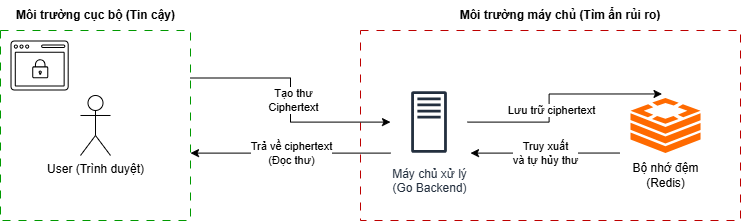
\includegraphics[width=\textwidth]{img/threat_model.png}
    \caption{Sơ đồ Luồng Dữ liệu (DFD) thể hiện Ranh giới Tin cậy (Trust Boundaries) trong kiến trúc Zero-Knowledge}
    \label{fig:threat_model_dfd}
\end{figure}

\textbf{Giả định cốt lõi về Ranh giới Tin cậy (Trust Boundary Assumption):} Mô hình đe dọa này được xây dựng dựa trên một giả thiết tối quan trọng: Trình duyệt web của người dùng (Client-side) phải là một môi trường an toàn và nguyên vẹn. Hệ thống Secret Letter không thể bảo vệ dữ liệu nếu bản thân thiết bị đã bị tổn hại từ trước (ví dụ: máy tính nhiễm mã độc, cài đặt các tiện ích mở rộng độc hại có khả năng đọc trộm bộ nhớ màn hình, hoặc hệ điều hành bị can thiệp). Đặc tính bảo mật đầu cuối chỉ phát huy tác dụng khi điểm cuối (Endpoint) thực sự nằm trong ranh giới an toàn.

\subsection{Spoofing (Giả mạo định danh)}

\textbf{Rủi ro:} Do đặc thù yêu cầu ẩn danh tuyệt đối, hệ thống chấp nhận rủi ro không thể xác thực danh tính người gửi (Spoofing) như một tính năng chủ đích (By-design). Tuy nhiên, kẻ tấn công có thể lợi dụng điều này để giả mạo hàng loạt người dùng nhằm phát tán thư rác (Spam) hoặc lạm dụng tài nguyên (Abuse).

\textbf{Biện pháp phòng ngừa:} Để ngăn chặn các cuộc tấn công lạm dụng, hệ thống triển khai cơ chế \textbf{Rate Limiting} nhiều lớp dựa trên địa chỉ IP (ví dụ: tạo tối đa 120 thư, giải mã 240 thư/giờ). Cần lưu ý sự đánh đổi (Trade-off): trong môi trường dùng chung IP (NAT) như trường học hoặc công ty, việc block IP có thể dẫn đến hiện tượng từ chối dịch vụ (DoS) cục bộ đối với các người dùng hợp lệ.

\subsection{Tampering (Can thiệp dữ liệu)}

\textbf{Rủi ro:} Kẻ tấn công, kể cả những quản trị viên có quyền truy cập vật lý vào cơ sở dữ liệu Redis, có thể cố tình chỉnh sửa nội dung bức thư (đã bị mã hóa) trước khi nó được gửi đến người nhận nhằm phá hoại tính toàn vẹn của dữ liệu.

\textbf{Biện pháp phòng ngừa:} Nhờ áp dụng thuật toán mã hóa \textbf{AES-256-GCM} (Galois/Counter Mode) cung cấp tính năng Authenticated Encryption, mọi nỗ lực thay đổi dù là một bit nhỏ nhất trên chuỗi \texttt{ciphertext} đều sẽ bị phát hiện trong quá trình giải mã tại trình duyệt. Cơ chế này đảm bảo nội dung thư nếu bị can thiệp sẽ hiển thị thông báo lỗi thay vì hiển thị dữ liệu sai lệch.

\subsection{Repudiation (Chối bỏ trách nhiệm)}

\textbf{Rủi ro:} Người gửi có thể phủ nhận việc đã gửi một bức thư có nội dung nhạy cảm, hoặc người nhận có thể phủ nhận việc đã đọc bức thư đó.

\textbf{Biện pháp phòng ngừa:} Rủi ro này thực chất được xem là một \textbf{tính năng} (Feature) của \textit{Secret Letter}. Dự án chủ trương thiết kế theo mô hình ẩn danh và không lưu vết (Anti-forensics). Hệ thống không lưu trữ địa chỉ IP, không ghi log thao tác cá nhân, và tự động hủy thư sau khi đọc. Do đó, việc không thể chứng minh ai là người gửi/người nhận là kết quả tất yếu của thiết kế Zero-Knowledge.

\subsection{Information Disclosure (Lộ lọt thông tin)}

\textbf{Rủi ro:} Nội dung bức thư có thể bị đánh cắp bởi tin tặc khi đang truyền tải trên mạng (Man-in-the-Middle) hoặc bị khai thác trực tiếp từ cơ sở dữ liệu máy chủ.

\textbf{Biện pháp phòng ngừa:} Đây là khía cạnh được hệ thống bảo vệ nghiêm ngặt nhất. Dữ liệu được bảo vệ bằng kênh truyền \textbf{TLS 1.3} chống nghe lén. Đột phá cốt lõi nằm ở kiến trúc \textbf{Client-Side Encryption (Mã hóa đầu cuối)}, trong đó khóa giải mã được truyền tải thông qua \textbf{URL Fragment} (\texttt{\#key}). Máy chủ chỉ nhận và lưu trữ bản mã vô nghĩa (\texttt{ciphertext}), hoàn toàn không có khả năng tự tiếp cận thông tin ngay cả khi bị tổn hại toàn diện.

\subsection{Denial of Service - DoS (Từ chối dịch vụ)}

\textbf{Rủi ro:} Hacker có thể liên tục gửi các yêu cầu tạo thư với Payload có kích thước khổng lồ nhằm làm cạn kiệt băng thông mạng, bộ nhớ RAM hoặc năng lực xử lý CPU của hệ thống.

\textbf{Biện pháp phòng ngừa:} Để chống lại các cuộc tấn công DoS, backend Golang được cấu hình với \texttt{http.MaxBytesReader} để ngắt kết nối ngay lập tức nếu dung lượng Request vượt quá giới hạn thiết kế. Đồng thời, cấu trúc dữ liệu trên Redis chia tách rõ ràng giữa Metadata (có kích thước cực nhỏ để truy vấn nhanh) và Payload, giúp hệ thống duy trì hiệu suất tra cứu ngay cả khi đang bị tấn công lưu lượng lớn.

\subsection{Elevation of Privilege (Nâng quyền hệ thống)}

\textbf{Rủi ro:} Kẻ tấn công có thể khai thác các lỗ hổng bảo mật trong mã nguồn Backend hoặc hệ điều hành để chiếm quyền điều khiển cao hơn, từ đó can thiệp vào tiến trình của ứng dụng.

\textbf{Biện pháp phòng ngừa:} Môi trường Backend được đóng gói bằng công nghệ Docker Container với tùy chọn \texttt{security\_opt: no-new-privileges:true} và giới hạn thư mục gốc ở chế độ \texttt{read\_only}. Việc thu hồi các quyền quản trị không cần thiết (Cap\_drop) giúp "giam lỏng" tiến trình ứng dụng, ngăn chặn khả năng kẻ tấn công vượt ngục (Container Escape) ra máy chủ vật lý.